\newcommand{\Release}{}
\newcommand{\Slide}{}
\newcommand{\PrintLecture}{1}
\newcommand{\PrintSolution}{0}
\newcommand{\MyCourse}{データサイエンスコース}
\newcommand{\MySemester}{春}
\newcommand{\MySubject}{ビジネス アナリティクス}
\newcommand{\MyClass}{第17回ー分類}% フォルダ名自動挿入

%
% 科目共通定義
%

\newcommand{\OpenIntro}
{\MyRef{OpenIntro Statistics}{https://www.openintro.org/book/os}}

\newcommand{\R}{\textbf{R}}
\newcommand{\RStudio}{\textbf{RStudio}}
\newcommand{\Excel}{\textbf{Excel}}
\newcommand{\cs}[1]{\textcolor{blue}{\texttt{#1}}} % Console prompt >

\newcommand{\ra}{\rightarrow}
\newcommand{\Ra}{\Rightarrow}

% Expectation E[X]
\def\E#1{E\big[#1\big]}
\def\S{\sum_{i=1}^n}

\newcommand{\B}{\hat{\beta}}
\newcommand{\SUM}{\sum_{i=1}^n}  % Summention from i=1 to n
\newcommand{\NH}{$\mathit{H}_0$} % Null hypthesis
\newcommand{\AH}{$\mathit{H}_1$} % Alternative hypothesis
\newcommand{\T}{\texorpdfstring{$t$}{}}% Student's t
\newcommand{\overtext}[3][1.5]{
  \mathrel{\overset{#2}{\scalebox{#1}[1]{$#3$}}}
}
\newcommand{\iid}{\overtext[2]{iid}{\sim}}
\newcommand{\convdist}{\overtext[2]{d}{\rightarrow}}
\newcommand{\convprob}{\overtext[2]{p}{\rightarrow}}
\newcommand{\as}[2]{\quad \text{as}\quad #1 \rightarrow #2}

\input{../../tex/hss_lualatex.tex}
\input{../../tex/hss_moodle.tex}
\input{../../tex/hss_beamer.tex}

\begin{document}

\maketitle

\section{小テスト(\MyClass)}

\begin{quiz}{\MyClass}

\QuizMultipleChoices
{
  回帰モデル全体の有意性を検定するときの検定統計量は何か?
}
{
  F検定統計量
}
{20}
{ z検定統計量}
{ t検定統計量}
{*F検定統計量}
{ $\chi^2$検定統計量}

\QuizMultipleChoices
{
  偏回帰係数(説明変数)の有意性を検定するときの検定統計量は何か?
}
{
  t検定統計量
}
{20}
{ z検定統計量}
{*t検定統計量}
{ F検定統計量}
{ $\chi^2$検定統計量}

\QuizShortAnswer
{
  カテゴリ変数やバイナリ変数(True/False)などの数値変数でない
  変数に対して0と1を用いて数値化した変数を\underline{     }という。
  空欄を埋めよ。
}
{
  ダミー変数
}
{20}
{ダミー変数}
{}
{}
{}

\QuizTrueFalse
{
  次の回帰モデルは有意水準5%で有意なモデルか?
  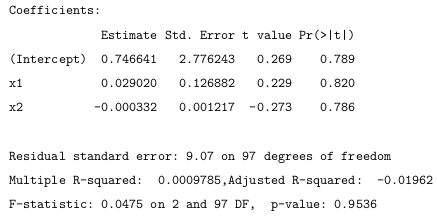
\includegraphics[width=\textwidth]{anl1.png}
}
{
  有効でない
}
{20}
{ 有意である}
{*有意でない}

\QuizTrueFalse
{
  説明変数$x2$の偏回帰係数は有意水準5%で有意か?
  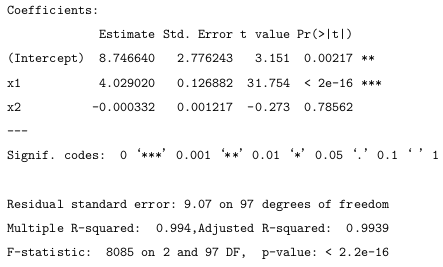
\includegraphics[width=\textwidth]{anl2.png}
}
{
  有効でない
}
{20}
{ 有意である}
{*有意でない}

\end{quiz}

\end{document}
